\chapter{Preliminares}
El desarrollo del presente trabajo descansa completamente sobre los hombros de tres conceptos: el operador de densidad, el principio de máxima entropía, y los modelos de grano grueso. En este capítulo se introducirán cada una de estas ideas. Primero, se discutirá el formalismo del operador de densidad, introducido mediante la necesidad de este a la hora de estudiar mezclas estadísticas de estados cúanticos. Luego se analizará el concepto de entropía en los contextos de las teorías de información tanto clásica como cúantica, a través del cual se derivará la expresión de la inferencia de máxima entropía de un sistema cuántico. Finalmente, se comentará sobre los modelos de grano grueso, como descripciones \textit{efectivas} de sistemas de dimensión alta, donde por \textit{efectivas} nos referimos a descripciones en las que no se tiene acceso a todos los grados de libertad del sistema. 

\ddnote{sería bueno mencionar efectivas en que sentido: cuando no se tiene acceso a todos los grados de libertad}. 

\acnote{¿Es suficente eso? Se profundiza más en la sección correspondiente.}

\ddnote{Aunque se profundice en la sección es bueno ser precisos aquí, pues esto es como una microintroducción al capitulo. Mejor pon algo sobre que no se tiene acceso a todos los grados de libertad, porque la realidad es que si se están tomando en cuenta, vamos, sabemos que existen.}

\acnote{¿Así queda?}

\section{El operador de densidad}

\subsection{Mezclas estadísticas}

\acnote{El siguiente párrafo ha sido iterado, solo notas}

En el contexto de la mecánica cuántica nos enfrentamos a dos tipos de probabilidades. La primera, la probabilidad cuántica, está codificada dentro de los vectores de estado que se utilizan para describir el estado en el que se puede hallar un sistema. Sin embargo, los vectores de estado no contemplan \ddnote{contemplan} el segundo tipo de probabilidad: la asociada a la ignorancia. Esta no es una probabilidad cuántica (aquella que se define como el valor absoluto al cuadrado de una amplitud de probabilidad) \ddnote{propongo añadir este paréntesis: (definida como el valor absoluto al cuadrado de una amplitud de probabilidad)}, sino una clásica. Por esto, y porque será particularmente útil para nuestro trabajo, introducimos el concepto del operador de densidad (también llamado, en el caso discreto, que es el que nos incumbe, matriz de densidad).

\acnote{El siguiente párrafo ha sido iterado, solo notas}

Supóngase que en lugar de estudiar un sistema que está completamente descrito por $\ket{\varphi}\in\hilbert_{n}$, con $\hilbert_{n}$ el espacio de Hilbert de dimensión $n$ \ddnote{añadamos: de dimensión $n$, \ie{}} $\hilbert_{n}=\Complex^{n}$; se trabaja con uno que está en el estado $\ket{\varphi_{i}}$ con probabilidad $p_{i}$, donde $\{\ket{\varphi_{i}}\}_{i=1}^n$ \ddnote{añadí rango de la $i$} es un conjunto no necesariamente ortogonal de estados de $n$ niveles $\ket{\varphi_{i}}\in\hilbert_{n}$, y $\{p_{i}\}_{i=1}^n$ \ddnote{añadí rango de la $i$} es un conjunto de números reales no negativos tales que $\sum_{i=1}^n p_{i}=1$ \ddnote{añadí rango de la $i$}.



\acnote{El siguiente párrafo ha sido iterado, solo notas}

De este sistema se dice que se halla en un estado de \textit{mezcla estadística}, y no debe confundirse con que el sistema se halle en una superposición de estados $\ket{\varphi_{i}}$ con coeficientes $\sqrt{p_{i}}$, ya que una superposición está bien determinada \ddnote*{determinado}{caracterizada}, y está completamente descrita por $\ket{\psi}=\sum_{i} e^{i \theta_i} \sqrt{p_{i}}\ket{\varphi_{i}}$ \ddnote{añadí fases a la ecuación, por generalidad}, mientras que la mezcla no lo está, ya que parte del elemento probabilístico \ddnote*{... :parte del elemento probabilístico...}{el elemento probabilístico} está asociado a un grado de ignorancia sobre la preparación del sistema. La mezcla estadística, en este sentido, toma en cuenta no sólo la probabilidad intrínseca a cada estado cuántico, sino una probabilidad clásica, $p_{i}$. Consideremos ahora un observable descrita por un operador hermítico $A$, se sabe que el valor de expectación del observable, con respecto a un estado $\ket{\varphi_{i}}$, está dado por $\expval{A}=\bra{\varphi_{i}}A\ket{\varphi_{i}}$. El valor esperado de dicho observable con respecto a la mezcla estadística será, justamente, el promedio de los valores esperados respecto a los estados cuánticos en la mezcla \ddnote*{promedio de los valores esperados respecto a los estados cuánticos en la mezcla}{combinación probabilística de los valores esperados respecto a los elementos de la mezcla}:
\begin{equation}
\expval{A}=\sum_{i}p_{i}\bra{\varphi_{i}}A\ket{\varphi_{i}}. \nonumber
\end{equation}
Pues bien, esta expresión puede ser manipulada a través de una base ortogonal $\{\ket{e_{k}}\}$ del espacio $\hilbert_{n}$:
\begin{align}
\expval{A}&=\sum_{i}p_{i}\bra{\varphi_{i}}A\ket{\varphi_{i}}\nonumber\\ 
&=\sum_{i,j,k}p_{i}\bra{e_{k}}\ket{\varphi_{i}}\bra{\varphi_{i}}\ket{e_{j}} \bra{e_{j}}A\ket{e_{k}} \nonumber
\end{align}
Esta es una suma sobre los elementos de la matriz del observador $A$ y las de las matrices definidas por $\dyad{\varphi_{i}}$. Agrupando la suma sobre $i$ y tomando en cuenta completez de la base $\{\ket{e_{j}}\}$,
\begin{align}
\expval{A}&=\sum_{j,k}\bra{e_{k}}\qty(\sum_{i}p_{i}\dyad{\varphi_{i}})\ket{e_{j}} \bra{e_{j}}A\ket{e_{k}}\nonumber\\
&=\sum_{k}\bra{e_{k}}\qty(\sum_{i}p_{i}\dyad{\varphi_{i}})A\ket{e_{k}}\nonumber\\
&=\Tr[\qty(\sum_{i}p_{i}\dyad{\varphi_{i}})A]\rlap{,}\nonumber
\end{align}
Con lo que la mezcla queda descrita por el operador de densidad $\rho$, definido según
\begin{equation}\label{eq:DensOpMix}
\rho=\sum_{i}p_{i}\dyad{\varphi_{i}}.
\end{equation}
\acnote{El siguiente párrafo ha sido iterado, solo notas}
Entonces podemos observar que es posible hallar el valor esperado de un observable respecto a un estado \ddnote*{estado}{sistema} utilizando el \ddnote*{utilizando el}{a través del} operador de densidad, cuya expresión está dada por \ddnote*{cuya expresión está dada por}{ que lo describe mediante}
\begin{equation}\label{eq:ExpValFromDensOp}
\expval{A}=\Tr(A\rho).
\end{equation}

El nombre ``operador de densidad'' puede resultar más claro comparando la ecuación (\ref{eq:ExpValFromDensOp}) con el valor esperado en estadística. Si $X$ es una variable aleatoria con dominio discreto $X=x_1,x_2,\dots$ y cuya distribución probabilidad es $p(x_k)$, entonces el valor esperado de una función $A$ de los valores de $X$ es
\begin{equation}
E[A]=\sum_{k} A(x_k) p(x_k).\nonumber
\end{equation}
\acnote{El siguiente párrafo no ha sido iterado}

\ddnote{estandarizé un poco la notación en la ecuación y texto anteriores}
\ddnote*{Este texto está raro. Ciertamente hay una analogía, pero no es claro que va por aquí}{Reconociendo que la operación traza no es sino la suma sobre los elementos diagonales de la matriz, es posible ver que la matriz de densidad ocupa un rol similar al de la función de densidad.}
Ahora, es necesario ser capaz de distinguir si un operador cualquiera corresponde a un operador de la forma (\ref{eq:DensOpMix}). De esta definición destilan dos propiedades que permiten reconocer si un operador arbitrario es un operador de densidad válido, o no \cite{Holevo}:
\begin{enumerate}
    \item $\Tr(\rho)=1$
    \item $\rho\geq 0$,
\end{enumerate}
\ddnote{donde $\rho\geq 0$ se define como $\bra{\varphi}\rho\ket{\varphi}\geq 0$ $\forall$ $\ket{\varphi}\in\hilbert_{n}$}.
La primera propiedad se deriva de la normalización de los estados $\ket{\varphi_{i}}$ que definen al sistema. La segunda establece que $\rho$ es una matriz positiva semidefinida y puede interpretarse como la necesidad de que la probabilidad de que el sistema descrito por $\rho$ se halle en el estado $\ket{\varphi}$ sea mayor o igual a $0$. Un operador es un operador de densidad si \ddnote*{en las definiciones basta solo el ``si''}{y solo si} cumple con estas propiedades. Por esto, estos dos puntos funcionan como una definición alternativa al operador de densidad.

\acnote{En el siguiente párrafo hay tres oraciones idénticas que me toca reescribir.}

A partir de este momento se asume que todos los espacios de Hilbert con los que se trabaja son complejos y de dimension finita. Esto es, son todos del tipo $\hilbert_{n}=\Complex^{n}$. Al conjunto de todos los operadores lineales acotados que actúan sobre un espacio $\hilbert_{n}$ se le denotará como $\mcB(\hilbert_{n})$. Luego, al conjunto de operadores lineales Hermitianos se le denotará mediante $\mcL(\hilbert_{n})$. Finalmente, al conjunto de operadores de densidad se le denotará mediante $\mcS(\hilbert_{n})$. Como nos concentramos en espacios de dimension finita, los operadores tienen representación matricial. Los términos \textit{matriz de densidad} y \textit{operador de densidad} se consideran intercambiables.



\subsection{Pureza}

La diferencia entre una mezcla estadística y una superposición puede no ser del todo clara. ¿Cómo son diferentes un sistema que tiene una probabilidad $p_{i}$ de hallarse en el estado $\ket{\varphi_{i}}$ y otro que se halla en una superposición de cada estado $\ket{\varphi_{i}}$ con coeficientes $\sqrt{p_{i}}$? 

Para responder, considérense dos sistemas de dos niveles. El primero puede hallarse en cualquiera de los siguientes estados
\begin{align}
    \ket{0}=\begin{pmatrix}
        1\\
        0
    \end{pmatrix} && \text{y} && \ket{1}=\begin{pmatrix}
        0\\
        1
    \end{pmatrix}\rlap{,}\nonumber
\end{align}
con la misma probabilidad $p=\frac{1}{2}$. Entonces el operador de densidad que describe al sistema es 
\begin{equation}
    \rho=\frac{1}{2}(\dyad{0}+\dyad{1})=\frac{1}{2}\Id_{2}.\nonumber
\end{equation}
Por otro lado, el segundo sistema se halla en una superposición de los mismos estados, con coeficientes $\sqrt{p}$. El operador de densidad que describe al segundo sistema es 
\begin{align}
    \dyad{\psi} && \text{con} && \ket{\psi}=\frac{1}{\sqrt{2}}(\ket{0}+\ket{1})\rlap{.}\nonumber
\end{align}
Es claro que $\ket{\psi}$ y $\rho$ no describen al mismo objeto, pues $\rho\neq\dyad{\psi}$. Si nos propusiéramos calcular la probabilidad de cada uno de hallarse en el estado $\ket{0}$ encontraríamos que
\begin{align}
    \bra{0}\rho\ket{0}=\frac{1}{2} && \text{y} &&\langle 0 \dyad{\psi} 0\rangle=\frac{1}{2}\rlap{.}\nonumber
\end{align}
y el resultado es el mismo si se hiciera con el estado $\ket{1}$. Parecería entonces que los sistemas se hallan en el mismo estado. Esto es falso. Si realizamos un cambio de base, de $\{\ket{1},\ket{2}\}$ a $\{\ket{+},\ket{-}\}$, donde
\begin{align}
    \ket{+}=\frac{1}{\sqrt{2}}\begin{pmatrix}
        1\\
        1
    \end{pmatrix} && \text{y} && \ket{-}=\frac{1}{\sqrt{2}}\begin{pmatrix}
        1\\
        -1
    \end{pmatrix}\rlap{,}\nonumber
\end{align}
y calculamos la probabilidad de que cada sistema se halle en el estado $\ket{+}$ encontraremos
\begin{align}
    \bra{+}\rho\ket{+}=\frac{1}{2} && \text{pero} &&\langle + \dyad{\psi} +\rangle=1\rlap{.}\nonumber
\end{align}
El segundo resultado es de esperarse, pues $\dyad{\psi}$ se halla en el estado $\ket{+}$. Por otro lado, el sistema $\rho$ siempre tendrá una probabilidad $\frac{1}{2}$ de hallarse en cualquiera de los dos elementos de cualquier base ortogonal que escojamos. La diferencia entre ambos sistemas es que el elemento probabilístico asociado a las mediciones sobre $\dyad{\psi}$ es de naturaleza cuántica, y viene de que el sistema se halla en una superposición de estados ortogonales, mientras que en el caso de $\rho$, el elemento probabilístico se debe a nuestra ignorancia sobre la preparación del estado \cite{Chuang}. El hecho de que hallemos que $\rho$ siempre tenga una probabilidad $\frac{1}{2}$ de hallarse en alguno de los dos elementos de cualquier base ortogonal es una propiedad del estado máximamente mezclado, que puede verse como un estado de cuya preparación somos máximamente ignorantes.

\acnote{La siguiente sección ha sido iterada, reescritura.}

\acnote{---------------- Obsoleto:}

\ddnote*{Observamos entonces que}{Vemos, pues, que} hay una diferencia fundamental entre los sistemas que pueden ser descritos por un vector de estado \ddnote*{este paréntesis está demás y puede crear confusión. Otra cosa, tienes corrector de ortografía en tu editor?, se han ido varios typos}{(para los que es posible contruir una matriz de densidad)}, y aquellos que no. \ddnote*{Esto se puede explicar de forma mucho mas simple, como diciendo: considere el caso en el que el sistema se encuentra en el estado $\ket{\varphi}$ con probabilidad igual a uno, \ie{} $\rho=\dyad{\varphi}$...}{Si para $\rho$ un operador de densidad,
\begin{equation}
    \rho=\sum_{i}p_{i}\dyad{\varphi_{i}},\nonumber
\end{equation}
se cumple que $\rho=\dyad{\varphi_{i}}$ $\forall i$,} entonces decimos que $\rho$ es un estado puro, y está completamente caracterizado por el vector de estado $\ket{\varphi}=\ket{\varphi_{i}}$. \ddnote*{Esto está escrito raro, mencionas la palabra proyector sin definirlo, pero despues defines $\rho$ usando la definición de proyector. Por fas dale una iterada}{Así, los estados puros (aquellos que están descritos por un vector de estado, i.e. su operador de densidad es un proyector) son los puntos extremos del conjunto convexo de operadores de densidad. Estos estados cumplen que
\begin{itemize}
    \item $\rho=\dyad{\psi}$ para algún vector de estado $\ket{\psi}$.
    \item $\rho=\rho^{2}$.
    \item $\Tr(\rho^{2})=1$.
\end{itemize}}
\ddnote{Cambiado $n$ por 2}
\acnote{---------------- Nuevo:}

Observamos entonces que hay una diferencia fundamental entre los sistemas que pueden ser descritos por un vector de estado y aquellos que no. Considérese el caso en que, dada la expresión \ref{eq:DensOpMix}, el estado del sistema es $\dyad{\varphi_{1}}$ con  probabilidad $p_{1}=1$, i.e. $\rho=\dyad{\varphi_{1}}$. En tal caso decimos que $\rho$ es un estado puro. Claramente, $\rho^{2}=\rho$. Esto hace de $\rho$ un proyector, de lo que se sigue que $\Tr(\rho^{1})=1$. 

Como en general se cumple que $\Tr(\rho^{2})\leq 1$, definimos a la pureza como una medida de que tan puro es un estado como \cite{Jaeger}
\begin{equation}
    \text{Pu}(\rho)=\Tr(\rho^{2}).\nonumber
\end{equation}
De esta definición es posible afirmar que
\begin{itemize}
    \item Un estado es puro si y sólo si $\text{Pu}(\rho)=1$.
    \item Para todo estado, $\frac{1}{n}\leq \text{Pu}(\rho)\leq 1$.
\end{itemize}

\subsection{Sistemas multipartitos}\label{sec:Ch1PartialTrace}
\ddnote{Sección pendiente por revisar}
Hasta ahora hemos hablado de sistemas descritos por operadores de densidad en $\densityspace{n}$, pero, ¿qué sucede si el sistema que estudiamos está conformado por dos subsistemas, cada uno descrito a través de sus respectivos espacios de Hilbert? Sean, pues, $A$ y $B$ dos sistemas con espacios de Hilbert $\hilbert^{A}$ y $\hilbert^{B}$, y sea $C$ un sistema compuesto por $A$ y $B$. Entonces el producto tensorial de los espacios $\hilbert^{A}$ y $\hilbert^{B}$ es otro espacio de Hilbert, uno asociado al sistema $C$:
 \begin{equation}
     \hilbert^{C}=\hilbert^{A}\otimes\hilbert^{B}.\nonumber
 \end{equation}
 La dimensión del espacio de Hilbert del sistema multipartito cumple
\begin{equation}
    \text{dim}(\hilbert^{C})=\text{dim}(\hilbert^{A})\text{dim}(\hilbert^{B}).\nonumber
\end{equation}
Si $A$ y $B$ representaran dos partículas diferentes, entonces $C$ representa a las partículas como conjunto, como sistema de dos partículas. Si cada una de las partículas puede ser descrita mediante un vector de estado, el estado del sistema es simplemente el producto tensorial de dichos vectores de estado:
\begin{equation}
    \ket{\psi^{A}}\otimes\ket{\psi^{B}}\in\hilbert^{C}\,\; \; \forall\ket{\psi^{A}}\in\hilbert^{A},\ket{\psi^{B}}\in\hilbert^{B}.\nonumber
\end{equation}
Si un estado puede escribirse como un producto tensorial de estados pertenecientes a los subsistemas del sistema multipartito, entonces se dice que es un estado \textit{producto} o \textit{separable}. Nótese que, en general, los estados del sistema compuesto no son estados separables. En realidad, dadas $\{\varphi_{i}^{A}\}$ y $\{\varphi_{j}^{B}\}$ bases ortonormales de los espacios $\hilbert^{A}$ y $\hilbert^{B}$ respectivamente, podemos escribir a todo estado puro $\ket{\psi^{C}}$ del sistema multipartito como
\begin{equation}
    \ket{\psi^{AB}}=\sum_{j,k}\alpha_{j,k}\ket{\varphi_{j}^{A}}\otimes\ket{\varphi_{k}^{B}}.\nonumber
\end{equation}
El significado físico de que un sistema se halle en un estado producto es que el sistema se halla en un estado en el que no hay correlaciones entre sus subsistemas (de esto que puedan separarse). Un estado que no puede separarse tiene cierto grado de entrelazamiento, y por esto deja de tener sentido hablar de vectores de estado individuales a cada partícula. Ahora, sean $G^{A}$ y $G^{B}$ dos operadores que actúan en $\hilbert^{A}$ y $\hilbert^{B}$ respectivamente, correspondientes a observables de cada subsistema. Entonces se cumple:
\begin{equation}
    G^{A}\ket{\psi^{A}}\otimes G^{B}\ket{\psi^{B}}=(G^{A}\otimes G^{B})\ket{\psi^{A}}\otimes\ket{\psi^{B}}.\nonumber
\end{equation}

¿Qué sucede si al científico no le interesa sino uno de los subsistemas? Es en este caso en el que surge el concepto de la matriz de densidad reducida. Si $\rho^{C}$ es la matriz de densidad del sistema compuesto por $A$ y $B$, entonces la matriz de densidad reducida del sistema $A$ es
\begin{equation}
    \rho^{A}=\Tr_{B}(\rho^{C}),\nonumber
\end{equation}
donde $\Tr_{B}$ representa la operación de traza parcial con respecto al subsistema $B$. Si la traza de $\rho^{C}$ es 
\begin{equation}
    \Tr(\rho^{C})=\sum_{j}\bra{\varphi^{C}_{j}}\rho^{C}\ket{\varphi^{C}_{j}},\nonumber
\end{equation}
para toda base ortonormal $\{\ket{\varphi^{C}_{j}}\}$ de $\hilbert^{C}$. Entonces, para toda base ortonormal $\{\ket{\varphi^{B}_{j}}\}$ de $\hilbert^{B}$  la traza parcial respecto a $B$ es \cite{Hardy}
\begin{equation}
    \Tr_{B}(\rho^{C})=\sum_{j}(\Id^{A}\otimes \bra{\varphi^{B}_{j}})\rho^{C}(\Id^{A}\otimes \ket{\varphi^{B}_{j}}).\nonumber
\end{equation}
Puede verse que el resultado de la operación es trazar sobre los elementos del sistema que no es de interés. La matriz reducida del sistema $A$, o traza parcial con respecto al sistema $B$, actúa como matriz de densidad de $A$, ya que contiene toda la descripción estadística de dicho subsistema.

\subsection{Evolución y parametrización}


\acnote{----Sección: Evolución de sistemas cerrados}

\acnote{
La evolución de un sistema cuántico cerrado descrito por un vector de estado está dada por la ecuación de Schrödinger,
\begin{equation*}
    i\hbar\frac{d}{dt}\ket{\psi(t)}=H\ket{\psi(t)},
\end{equation*}
cuya solución formal está dada en términos de un operador unitario $U(t,t_{0})$ según
\begin{align*}
    \ket{\psi(t)}=U(t,t_{0})\ket{\psi(t_{0})} && \text{con} && U(t,t_{0})=e^{-iH(t-t_{0})/\hbar}\rlap{.}
\end{align*}
Pues bien, los postulados de la mecánica cuántica pueden adaptarse al formalismo de operadores de densidad. De la ecuación de Schrödinger se sigue que la evolución de un sistema descrito por un operador de densidad $\rho$ está descrita por ecuación de Liouville-von Neumann,
\begin{equation*}
    i\hbar\frac{d}{d t} \rho(t)=[H,\rho(t)].
\end{equation*}
De la misma forma que antes, la solución queda expresada en términos de un operador unitario,
\begin{equation*}
    \rho(t)=U(t,t_{0})\rho(t_{0})U^{\dagger}(t,t_{0}).
\end{equation*}
}

\acnote{----Sección: evolución de sistemas abiertos}

\acnote{Considérese, en cambio, que el sistema de interés $\rho_{S}$ se halla acoplado a un entorno $\rho_{E}$ y que, inicialmente, el conjunto de estos dos conforma un sistema cerrado descrito por el operador de densidad $\rho(0)=\rho_{S}(0)\otimes\rho_{E}$. Esta condición inicial está justificada experimentalmente: una medición proyectiva sobre el sistema de interés proyecta al sistema a un estado factorizable, así que estos estados son siempre preparables. Como el sistema es cerrado, este evoluciona siguiendo la ecuación de Liouville-von Neumann,
\begin{align*}
    i\hbar\frac{d}{d t} \rho(t)=[H,\rho(t)] && \text{con} && \rho(0)=\rho_{S}(0)\otimes\rho_{E}\rlap{,}
\end{align*}
cuya solución formal es 
\begin{equation*}
    \rho_{S}(t)=\mcE_{t}(\rho(0)),
\end{equation*}
donde $\mcE_{t}$ es un canal cuántico para cualquier $t$, y $\mcE_{0}=Id$. El formalismo cuántico queda fuera del alcance de este trabajo, y sin entrar en más detalle, basta con señalar que los canales cuánticos son aplicaciones lineales de $\mcB(\hilbert_{n})$ en $\mcB(\hilbert_{m})$ que cumplen que  [LISTA PROPIEDADES DE CANALES].
Es particularmente interesante señalar que dado un canal cuántico, por el teorema de Stinespring...}

\subsubsection{La evolución del operador de densidad}

Los postulados de la mecánica cuántica pueden adaptarse al formalismo de operadores de densidad. En particular, reconociendo que la evolución de un sistema cuántico cerrado descrito por un vector de estado $\ket{\psi}$\ddnote{, está dada} por la ecuación de Schrodinger  \ddnote{Aquí no es tan necesario citar, ya es como citar a Newton cada vez que escribes una derivada. Si citas a alguien para cosas más trascendentes, mejor cita al autor del paper orginal} \acnote{cita removida},
\begin{equation*}
    i\hbar\frac{d}{dt}\ket{\psi(t)}=H\ket{\psi(t)},
\end{equation*}
\ddnote*{y cuya solución formal está dada en terminos de un operador unitario}{puede ser representada a través de un operador unitario} $U(t,t_{0})$ según
\begin{align*}
    \ket{\psi(t)}=U(t,t_{0})\ket{\psi(t_{0})} && \text{con} && U(t,t_{0})=e^{-iH(t-t_{0})/\hbar}\rlap{,}
\end{align*}
\ddnote*{Evita este tipo de expresiones, en la física matemática las cosas son o no son. Propongo algo como: Es directo probar,  a partir de la ecuación de Schrödinger, que el operador de densidad evoluciona de acuerdo a la siguiente expresión (en la que aparece el Hamiltoniano), cuya solución formal es (luego pones la expresión en términos de la unitaria)}{es posible afirmar que dado un operador de densidad $\rho(t_{0})$, este evoluciona de acuerdo a
\begin{equation*}
    \rho(t)=U(t,t_{0})\rho(t_{0})U^{\dagger}(t,t_{0}).
\end{equation*}
Derivando respecto al tiempo, se obtiene la \textit{ecuación de Liouville-von Neumann}, que corresponde a la ecuación de evolución para operadores de densidad,
\begin{equation}\label{eq:vonNeumann}
    i\hbar\frac{d}{d t} \rho(t)=[H,\rho(t)]
\end{equation}
}
Si, por otro lado, se piensa que el sistema estudiado se halla acoplado a un entorno (de tal forma que el conjunto sea un sistema \ddnote*{bipartito}{multipartito}), y que el conjunto de estos dos conforma un sistema cerrado descrito por el operador de densidad $\rho$, \ddnote*{evita el ``es posible afirmar'', me parece una expresión débil para conceptos bien determinados. Propongo: es decir, $\rho$ evoluciona de forma unitaria [cita la ecuación pertinente]}{entonces es posible afirmar que la evolución conjunta es de naturaleza unitaria.} De acuerdo con nuestra discusión sobre sistemas \ddnote*{biparititos}{multipartitos}, el sistema y el entrono se ven desritos por operadores de densidad
\begin{align*}
    \rho_{S}=\Tr_{E}(\rho) & & \text{y} & & \rho_{E}=\Tr_{S}(\rho)
\end{align*}
respectivamente. Siendo $\rho_{S}$ el estado de interés, podemos trazar ambos lados de la ecuación de Liouville-von Neumann para hallar una ecuación \ddnote*{Esta discusión tiene varios problemas importantes, lo hablamos en la reunión}{de la dinámica del sistema,
\begin{align*}
    i\hbar\frac{d}{d t} \rho_{S}(t)=\Tr_{S}([H,\rho(t)])
\end{align*}
en donde el claro problema es que el lado derecho de la ecuación, que está en términos de el conjunto y no del sistema de interés. La dinámica del sistema $S$ no será, en general, unitaria, y las diferentes aproximaciones a la dinámica de sistemas abiertos, entre las que se hallan las ecuaciones maestras, quedan por fuera del alcance de este trabajo.}


\subsubsection{Parametrización del operador de densidad}
\acnote{Esta parte aún la tengo que iterar}

\acnote{Es común escoger alguna base Hermítica para poder parametrizar a las matrices de densidad. El beneficio de hacer esto es que, por ser $\mcS(\hilbert_{n})$ un subconjunto de $\mcL(\hilbert_{n})$, dicha parametrización será lineal, y aún más: los parámetros serán cantidades medibles en el laboratorio. Esto significa que, realizando mediciones de forma adecuada, es posible reconstruir el estado de un sistema [cita]. Una elección común de base son las matrices generalizadas de Gell-Mann, junto a la matriz identidad.}

\acnote{Remplaza:-------}
\ddnote*{la base es hermitiana, el espacio no, lo hablamos en la reunión}{Cualquier matriz de densidad puede descomponerse en términos de una base del espacio de matrices hermitianas de $n\times n$.} \ddnote*{Tengo entendido que la identidad es también un generador de SU(2), checa bien esto}{Una elección común de base para el espacio es el de los generadores $\{\varsigma_{k}\}$ del grupo $\text{SU}(n)$, junto a la matriz identidad $\Id_{n}$}. Esto es particularmente útil, \ddnote*{ya que}{pues }permite parametrizar a las matrices de densidad de forma vectorial \cite{Bruning}. 
\acnote{---------fin}


\acnote{En efecto, sea $\{\varsigma_{k}\}$ el conjunto de matrices generalizadas de Gell-Mann que generan a $\text{SU}(n)$ y}
%En efecto, sea $\{\varsigma_{k}\}$ un conjunto de generadores de $\text{SU}(n)$ y 
$\rho$ una matriz de densidad $\rho\in\mcS(\hilbert_{n})$. Entonces $\rho$ está completamente descrita por el vector generalizado de Bloch de dimensión $2n^{2}-1$, $\vec{\gamma}$ definido según
\begin{equation}
    \rho=\frac{1}{n}\Id_{n}+\frac{1}{2}\vec{\gamma}\cdot\vec{\varsigma}.
\end{equation}
Si $n=2$, los generadores corresponden a las matrices de Pauli $\sigma_{i}$. En tal caso, el conjunto de vectores de Bloch corresponde a la bola unitaria tridimensional, con los estados puros en la superficie y las mezclas en el interior. Para casos en los que la dimensión es una potencia de $k$, es posible obtener nuevos generadores a través de los productos tensoriales de las matrices de Pauli consigo mismas y con la matriz identidad correspondiente. El caso $n=4$, por ejemplo \cite{Chuang}:
\begin{equation}\label{eq::BlochParametrization4}
    \rho=\frac{1}{4}\sum_{i,j}\gamma_{ij}\sigma_{i}\otimes \sigma_{j} \ \ i,j\in\{0,1,2,3\},
\end{equation}
donde $\sigma_{0}=\Id$ y 

\acnote{
\begin{equation*}
        \gamma_{i.j}=\Tr(\sigma_{i}\otimes \sigma_{j}\rho).
\end{equation*}
Obsérvese que, como se mencionó previamente, debido a que los parámetros $\gamma_{i.j}$ son cantidades medibles, esto junto a la ecuación [2.4] (meter referencia bién) permite reconstruir el estado del sistema.}\ddnote{...son promedios de las observables $\sigma_i \otimes \sigma_j$... obsérvese que esto junto a la ecuación [tal], permite reconstruir el estado cuántico $\rho$, a esto se le llama \textit{tomografía cuántica} etc.}

\section{Entropía}
\subsection{Entropía de Shannon}
A finales de los años cuarenta, Claude Shannon se preguntaba sobre una medida de la \textit{incertidumbre}, o de la \textit{información} asociada a un proceso cuyo resultado estuviera descrito por una variable aleatoria $X$ con distribución de probabilidad $p(x_{i})$.

La cantidad de información provista por el producto de un experimento depende de la probabilidad asociada a dicho suceso. Al tirar un dado, por ejemplo, saber que un número no cayó es mucho menos informativo que conocer que dicho número cayó, ya que cada número tiene una probabilidad de $\frac{5}{6}$ de no caer, pero sólo $\frac{1}{6}$ de caer. Con la misma línea de razonamiento, conocer el resultado de un evento que ocurre con probabilidad $p=1$ no transmite ninguna información. Si a cada valor de $X$ se le puede asociar una cantidad de información, entoces debe poder calcularse la cantidad de información promedio: esta es la medida que buscaba Shanon. La forma de esta medida, denótese $S(p)$, vino de las propiedades que el matemático estadounidense afirmó que debía cumplir \ddnote*{\cite{Shannon,Wilde}}{\cite{Shannon} \cite{Wilde}}:
\begin{enumerate}
    \item $H(p)$ debe ser continua en $p$
    \item $H(p)$ debe ser una función creciente monotónica de $n$ cuando $p_{i}=\frac{1}{n}$
    \item si $X$ e $Y$ son procesos independientes, $H(p_{X}(x_{i}),p_{Y}(y_{j}))=H(p_{X}(x_{i}))+H(p_{Y}(y_{j}))$
\end{enumerate}
\ddnote{faltan puntos en los items}
\acnote{no estoy tan seguro de que las listas lleven puntos}
y demostró que
\begin{equation}\label{eq:ShannonEntropy}
    H=-k\sum_{i}p(x_{i})\log{p(x_{i})}.
\end{equation}
Fue a través de discusiones con Von Neumann que Shannon descubrió que su medida ya era ampliamente utilizada en física, y que llevaba el nombre de \textit{entropía} \cite{McIrvine}.

La entropía de Shannon (\ref{eq:ShannonEntropy}) es máxima para distribuciones equiprobables. En el tiraje de un dado bien balanceado, no es posible tener más seguridad de que caiga un número que otro: la incertidumbre, o la entropía, es máxima.

En teoría de información clásica, la entropía de Shannon se suele estudiar como la cantidad promedio de bits requerida para trasmitir un mensaje. Un ejemplo común es de la cadena de caracteres, cada caracter pudiendo ser A, B, C o D. Si la probabilidad de cada caracter sea cualquiera de las cuatro letras es $\frac{1}{4}$ (máxima entropía), entonces se requieren dos bits para indicar el valor de cada caracter en la cadena (cada letra codificada como 00, 01, 10, o 11). Sin embargo, si las probabilidades son $p(A)=\frac{1}{2}$, $p(B)=\frac{1}{4}$, $p(C)=\frac{1}{8}$, $p(D)=\frac{1}{8}$, pueden asignarse los valores 1, 10, 110, 111, a cada letra, respectivamente. En promedio, cada letra requerirá $1.75$ bits para ser transmitida \cite{Chuang}. 

\subsection{Entropía de von Neumann}

La entropía de von Neumann, a pesar de haber sido obtenida veinte años antes, puede verse como la extensión cuántica de la entropía clásica de Shannon. Von Neumann introdujo el concepto del operador de densidad de forma independendiente a L. Landau, y definió la entropía $S$ asociada a un sistema descrito por un operador de densidad $\rho$ como \cite{vonNeumann}
\begin{equation}\label{eq:VonNeumannEntropy}
    S(\rho)=-\Tr(\rho\ln{\rho}).
\end{equation}
\acnote{El siguiente párrafo ha sido iterado, solo notas}

La entropía de von Neumann puede interpretarse de manera similar a la entropía de Shannon. Si se desea transmitir un qubit preparado como $\ket{\psi_{i}}$ con probabilidad $p_{i}$, entonces el operador de densidad que representa al estado enviado es justamente $\rho=\sum p_{i}\dyad{\psi_{i}}$. La cantidad de información recibida, o la incertidumbre sobre el qubit enviado, es justamente $S(\rho)$. Debe hacerse hincapié en el hecho que la entropía de un sistema cuántico debe es fundamentalmente diferente a la de un sistema clásico. El sistema cuántico presenta dos tipos de incertidumbres: la incertidumbre clásica, relacionada a nuestra falta de conocimiento relativa a un sistema, y la incertidumbre cuántica, una propiedad intrínseca a los sistemas ondulatorios, matemáticamente expresada a través del Principio de Incertidumbre de Heisenberg \cite{Wilde}.

La entropía de von Neumann de un sistema descrito por un operador de densidad $\rho\in\mcS(\hilbert_{n})$ tiene las siguientes propiedades \cite{Chuang}:
\acnote{Lista iterada parcialmente, solo notas, a discutir en reunión}
\begin{enumerate}
    \item La entropía puede escribirse en términos de los eigenvalores de $\rho$, $\eta_{j}$, como $S(\rho)=-\sum_{j}\eta_{j}\ln{\eta_{j}}$. \ddnote{Por fas añadé: lo que coincidé con la entropía de Shannon en un escenario en el que se envían los eigenestados de $\rho$, perfectamente distinguibles por ser ortogonales entre sí, con probabilidad $\eta_j$. Si tienes problemas con esto, lo platicamos.}
    \item La entropía es no negativa, y es nula si y sólo sí $\rho$ es de la forma $\dyad{\psi}$ con $\ket{\psi}\in\hilbert_{n}$
    \item La entropía es máxima cuando $\rho=\frac{1}{n}\Id_{n}$, \ddnote{por fas explica este estado y por que es el que debe tener entropía máxima}, y $S(\rho)=n$. Esto es de esperarse, de acuerdo con nuestra discusión previa, el estado máximamente mezclado es aquel del que somo máximamente ignorantes, y por lo mismo debe ser el que tiene la máxima entropía (recordando a la entropía como medida de incertidumbre).
    \item La entropía de un estado producto es igual a la suma de las entropías de cada factor, $S(\rho_{A}\otimes\rho_{B})=S(\rho_{A})+S(\rho_{B})$. \notaAd{En ningún lado he visto que los factores tengan que tener la misma dimensión, ¿por qué está mal, entonces, comparar las entropías pre y post CG?}\ddnote{Ojo que la cuestión es diferente. Aquí estás hablando de factores de un mismo sistema. Con CG hablamos de comparar dos sistemas, es como comparar la entropía de un dado de 6 caras con una moneda.}
    \item \notaAd{Hay algunas otras propiedades que aún no he terminado de entender, ni sé aplicar}\ddnote{En la siguiente reunión me las dices y las platicamos.}
\end{enumerate}
\section{El principio de máxima entropía}\label{sec:CH1MaxEnt}

\subsection{El principio de máxima entropía clásico}

Si se nos informa que el valor esperado de tirar un dado de seis caras particular es $3.5$. ¿Cuál es la probabilidad asociada a cada cara del dado? En principio, el problema no puede resolverse, porque la distribución de probabilidad que da como resultado el valor esperado de $3.5$ no es única. Sería igual de válido asumir que el dado está pesado de tal forma que cae la mitad de veces en $2$, y la otra mitad de veces en $5$, que suponer que todos los valores tienen una probabilidad $\frac{1}{6}$. La segunda opción, claro, parecería la más judiciosa. Esta opción es también la que más incertidumbre sobre cada resultado tiene asociada, y la que menos suposiciones sobre los pesos del dado hace. Aún más importante, asumir que todos los valores son igualmente probables equivale a escoger la distribución de probabilidad que maximiza la entropía.

El principio de máxima entropía fue introducido por E. T. Jaynes en 1957. En su artículo, \textit{Information Theory and Statistical Mechanics}: Jaynes afirma que la distribución de probabilidad que maximice la entropía es la mejor estimación que se puede hacer a través de la información disponible, independientemente de si las predicciones coinciden, o no, con los resultados experimentales \cite{JaynesI}. La estimación obtenida a través de la maximización de la entropía es, además, aquella que introduce la menor cantidad de información externa al sistema.

Jaynes relaciona la teoría de información clásica con la mecánica estadística no por la simple coincidencia en la forma de las entropías de Shannon y de Gibbs, sino a través de una reinterpretación de la mecánica estadística como una forma de inferencia estadística. En este contexto, viendo la entropía física como una medida de la incertidumbre asociada a una distribución de probabilidad, una distribución $p$ que no maximice la entropía, es una distribución que introduce información arbitraria no incluída en las hipótesis iniciales. En efecto, el problema de hallar una distribución de probabilidad adecuada es también un problema de contaminación de la información accesible. Esta contaminación proviene de suposiciones arbitrarias, y sin sustento físico, que pueden hacerse sobre el sistema. Utilizar el principio de máxima entropía permite hallar la distribución de probabilidad menos sesgada posible.

Supóngase que los resultados de un proceso corresponden a los valores $x_{i}$ de una variable aleatoria $X$. Sean, además $f_{i}$, funciones sobre $X$, de las que conocemos su valor esperado. La información accesible se puede escribir como el conjunto de restricciones
\begin{equation}\label{eq:JaynesRestrictions}
    \expval{f_{j}(x)}=\sum_{i}p(x_{i})f_{j}(x_{i}).
\end{equation}
Buscamos $p$ tal que maximice la etropía de Shannon (\ref{eq:ShannonEntropy}), sujeta a las restricciones experimentales (\ref{eq:JaynesRestrictions}). Para esto, utilizamos el método de multiplicadores de Lagrange. A las restricciones anteriores debe añadirse 
\begin{equation}\label{eq:NormalizationRestriction}
    \sum_{i}p(x_{i})=1.
\end{equation}
Pedimos que la derivada con respecto a la distribución $p$ de la Lagrangiana
\begin{equation*}
    \mcL=-H(p)+\sum_{j}\lambda_{j}\qty(\sum_{i}p(x_{i})f_{j}(x_{i})-\expval{f_{j}(x)})+\mu\qty(\sum_{i}p(x_{i})-1)
\end{equation*}
se anule. En esta ecuación, $\lambda_{j}$ es el multiplicador de Lagrange que pesa a la $j$-ésima restrición. Derivando e igualando a cero se obtiene que
\begin{gather*}
    \frac{\partial \mcL}{\partial p}=k(1+\log{p(x_{i})})+\sum_{j}\lambda_{j}f_{j}(x_{i})+\mu=0\\
    \Rightarrow p(x_{i})=\exp[-(1+\frac{\mu}{k})-\frac{1}{k}\sum_{j}\lambda_{j}f_{j}(x_{i})].
\end{gather*}
Esta es la distribución que maximiza a la entropía. Respecto a los multiplicadores de Lagrange, nótese que por la restricción (\ref{eq:NormalizationRestriction}) se cumple que
\begin{equation*}
    \frac{1}{e^{-(1+\mu)}}=\sum_{i}\exp[-\frac{1}{k}\sum_{j}\lambda_{j}f_{j}(x_{i})].
\end{equation*}
A partir de esta relación se define a la función de partición,
\begin{equation*}
    Z=\sum_{i}\exp[-\frac{1}{k}\sum_{j}\lambda_{j}f_{j}(x_{i})],
\end{equation*}
que satisface
\begin{equation*}
    \expval{f_{j}(x)}=-\frac{\partial}{\partial \lambda_{j}}\ln{Z}.
\end{equation*}
Considerando lo anterior, el estimado para la distribución de probabilidad que maximiza la entropía, y que es compatible con las restricciones (\ref{eq:JaynesRestrictions}) tiene la forma 
\begin{equation}\label{eq:MaxEntDist}
    p(x_{i})=\frac{1}{Z}\exp[-\frac{1}{k}\sum_{j}\lambda_{j}f_{j}(x_{i})].
\end{equation}

\subsubsection{El estimado de máxima entropía en mecánica estadística}

\acnote{Creo que así queda mejor está sección}

=============================================

El método anterior puede aplicarse a toda una variedad de sistemas y procesos. Considérese, pues, de un conjunto de $N$ partículas idénticas pero distinguibles de energías $\epsilon_{i}$, del cual únicamente conocemos la energía promedio $E$, y que se halla en equilibrio térmico con un entorno que actúa como baño de calor a una temperatura $T$. Nos interesa conocer la distribución de probabilidad de los posibles microestados $\epsilon_{i}$. Según lo discutido previamente, se busca maximizar la entropía,
\begin{equation}\label{eq:GibbsEntropy}
    S_{G}=-k_{B}\sum_{i}p(x_{i})\log{p(x_{i})},
\end{equation}
que es la entropía de Gibbs, con $k_{B}$ la constante de Boltzmann. Continuando con el procedimiento, se halla que la distribución de máxima entropía compatible con la restricción $\expval{\epsilon}=E$ es
\begin{equation}\label{eq:Boltzmann}
    p(x_{i})=\frac{e^{-\frac{\lambda}{k_{B}}\epsilon_{i}}}{Z}.
\end{equation}
Para discernir el significado físico de dicho resultado, se puede sustituir esta distribución en (\ref{eq:Boltzmann}), para encontrar que
\begin{equation}
    S_{G}=\lambda\expval{\epsilon}+k_{B}\ln{Z}.
\end{equation}
Recordando que, en la teoría de la termodinámica se define a la temperatura como el inverso del cambio de la entropía según la energía, se halla el significado físico del multiplicador de Lagrange, pues se tiene que cumplir que
\begin{equation*}
    \lambda=\frac{1}{T}.
\end{equation*}

=============================================

Si aplicáramos el principio de máxima entropía a un sistema físico \ddnote{Ten cuidado aqui, uno siemple aplica esto a sistemas fisicos, la particularidad a resaltar aqui es que se trata de un sistema en equilibrio termico.} como, por ejemplo, el de un conjunto de $N$ partículas idénticas pero distinguibles de energías $\epsilon_{i}$, del cual únicamente conocemos la energía promedio $E$, nos encontraríamos con que
\begin{equation}\label{eq:Boltzman}
    p(x_{i})=\frac{e^{-\lambda\epsilon_{i}}}{Z},
\end{equation}
que reconocemos como la distribución de Boltzmann, en la que $\lambda=\beta=\frac{1}{k_{B}T}$. \ddnote{La idea aqui es que no solo sabemos el promedio de la energia está fijo en la teória), sino que las fluctuaciones alrededor de ese valor son negligibles, debido a que el sistema está en equilibrio térmico y el sistema está además en el límite termódinamico. Bajo esas condiciones es que uno puede hacer la identificación del multiplicador de Lagrange con la temperatura. Dale una leídita al Greiner.}
\subsection{Extensión a la mecánica cuántica}

En su segundo artículo, Jaynes extiende el Principio de máxima entropía a la mecánica cuántica \cite{JaynesII}. Para esto, identificamos al operador de densidad cuántico como la distribución de probabilidad que buscamos hallar, dados algunos resultados experimentales.

Sean, pues, $\hat{A}_{j}$ $m$ operadores hermitianos que operan sobre $\hilbert_{n}$, con $m<n^{2}-1$, de tal forma que formen un conjunto no tomográficamente completo. Dados sus valores esperados,
\begin{equation}\label{eq:QuantumRestrictions}
    \expval{\hat{A}_{j}}=\Tr(\rho \hat{A}_{j}),
\end{equation} 
nos interesa hallar qué operador de densidad es el que mejor descibe a nuestro sistema. Invocando el Principio de máxima entropía, buscamos aquel que maximiza la entropía de von Neumann (\ref{eq:VonNeumannEntropy}). bajo las restricciones (\ref{eq:QuantumRestrictions}) además de
\begin{equation}\label{eq:TraceRestriction}
    \Tr(\rho)=1.
\end{equation}
Una vez más se utiliza el método de los multiplicadores de Lagrange, de manera análoga a como se hizo en el caso clásico. El estado de máxima entropía compatible con las observaciones experimentales es entonces
\begin{equation*}
    \rho=\frac{e^{-\sum_{j} \lambda_{j} \hat{A}_{j}}}{Z}.
\end{equation*}
\subsubsection{Caso termodinámico cuántico}
\notaAd{Conocemos $\expval{H}$. El estado de máxima entropía es un estado estacionario. Entonces conmuta con $H$ y comparten eigenbase. ¿Los observables son $H_{kk}$ en la base diagonal? Asumo que esto es los valores esperados respecto a los elementos de la eigenbase. Entonces
\begin{equation*}
    \lambda_{k}=\frac{e^{-\beta H_{kk}}}{Z}
\end{equation*}
¿Y este es el k-ésimo eigenvalor de $\rho$?}
\ddnote{Si, $\lambda_k$ es el $k$-ésimo eigenvalor de $\rho$, pero eso tu lo impones, pues usas la eigenbase de $\rho$. De pronto expliqué esto un poco revuelto. Naturalmente uno puede sustituir $H_{kk}$ por $E_k$ (los eigenvalores de $H$) y la cosa es más clara. La observable es la misma de arriba, la energía $E=\sum_l \lambda_k E_k$, de pronto también te expliqué esto con las patas. La idea entonces, es que una vez tengas los $\lambda_k$, resueltos, uses la notación bra-ket para escribir al final el resultado con los operadores (ahora si independiente de labase).} 
%
\ddnote{Para el argumento de que $[H,\rho]=0$ no olvides usar el argumento de la estacionariedad de $\rho$, dado que no solo se considera un estado de maxima entropía, sino termodinámico como en el caso clásico, uno espera que el estado no cambie respecto al tiempo, por lo tanto conmuta con el Hamiltoniano. Ese es el truco para sacar este estado. También puedes mencionar que siempre que tengas una colección de observables $A_k$ que conmutan con $\rho$ y conoces sus promedios, también puedes calcular el estado MaxEnt. El caso complicado, y es el que mencionarás que derivan en la referencia y que aquí solo mencionamos el resultado, es el caso cuando los $A_k$ no conmutan con $rho$.}

\ddnote{Por fas comienza a usar el comando siguiente:}
\acnote{nota de Adán aquí}
\section{Modelos de grano grueso}\label{sec:Ch1CG}

\subsection{Descripciones efectivas}

\acnote{Sección iterada: reescritura, requiere revisión.}

 \acnote{Sección iterada: notas}

En nuestro día a día no podemos procesar toda la información de todos los sistemas con los que interactuamos: no nos preocupa la energía cinética individual de cada una de las moléculas de agua presente en cada una de las gotas que caen sobre nosotros, sino qué tan caliente o frío parece el chorro que sale de la llave. Una descripción de \textit{grano grueso} es aquella que no toma en cuenta todos los detalles de un sistema o fenómeno. Estas particularidades microscópicas suelen omitirse ya sea por la incapacidad del observador de procesar toda la información asociada a estas, o de no tener acceso a todos los grados de libertad de dicho sistema.

El conjunto de variables termodinámicas de un sistema en equilibrio térmico puede verse como una descripción efectiva de una realidad microscópica subyacente. En este sentido, de la mecánica estadística pueden obtenerse estas variables termodinámicas como promedios de propiedades microscópicas. A las colisiones de un número estadísticamente significativo de partículas contra las paredes de un objeto se les puede promediar y reducir a una única variable: presión. De manera similar, la temperatura de un gas ideal se relaciona con la energía cinética de las partículas de este explícitamente a través de un promedio utilizando la distribución de Boltzmann. En efecto, 
\begin{equation}
    T=\frac{1}{k_\text{B}}\frac{2}{3}\expval{E_{\text{cin}}}.
\end{equation}
\begin{figure}[ht]
    \centering
    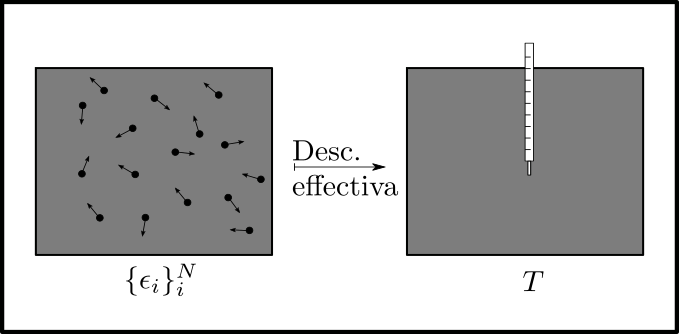
\includegraphics[width=0.6\linewidth]{chapter1/figures/CGT.png}
    \caption{Reducir las energías cinéticas individuales de $N$ partículas a un temperatura es un modelo de grano grueso}
    \label{fig:KtoT}
\end{figure}

En mecánica estadística se utiliza la estadística para pasar de una descripción fina a una gruesa, en la que cantidades arbitrariamente grandes de variables son sustituidas por distribuciones de probabilidad.

Los modelos de grano grueso son útiles porque permiten hacer predicciones sin tener que lidiar con cantidades de información que pueden ser no manejables, o simplemente no accesibles. Por esta razón, los modelos de grano grueso son comunes en física-química \cite{PhysChemI,PhysChemII,PhysChemIII} \acnote{revisar bien estos artículos}.


\subsection{Grano grueso en mecánica cuántica}

\acnote{Sección iterada, notas}

En el contexto de la mecánica cuántica, un modelo de grano grueso puede obtenerse trazando sobre un subsistema del sistema de interés. Es importante notar que el subsistema ignorado no es necesariamente una parte que puede ser separada del sistema, como en el caso de dos partículas, sino que puede representar otros grados de libertad del sistema que se deciden ignorar, por ejemplo, al describir un ión atrapado en una trampa magnetoóptica, una opción es ignorar los grados de libertad espaciales y quedarse solo con el espín total del ión \cite{Fox}. Ahora, la separación sistema-entorno no es siempre posible \cite{Macro-To-Micro}, por lo que nos limitamos a los casos en los que los grados de libertad ignorados pueden trazarse a través de la operación de traza parcial, como se discutió en la sección \ref{sec:Ch1PartialTrace}.

Un ejemplo sencillo de un modelo de grano grueso es el de un sistema de dos partículas, del cual únicamente nos importa una. En dicho caso, el modelo puede consistir en estudiar únicamente al operador de densidad reducido correspondiente a la partícula de nuestro interés. De forma general en el contexto de este trabajo, el modelo de grano grueso consiste en reducir la dimensión del sistema estudiado. En nuestro contexto, una aplicación de grano grueso $\Lambda$ es tal que manda a un operador de densidad $\varrho\in\densityspace{n}$ a algún otro operador de densidad $\rho\in\densityspace{m}$ con $m<n$. Esto es:
\begin{align}
    \mcF:\densityspace{n}\to \densityspace{m}, n>m\nonumber
\end{align}

\newpage